\section{Implementación} \label{sec:implementacion}
Aplicando la metodología \textit{benchmarking}, planteando posibles estrategias bajo parámetros diferentes y la revisión continua de expertos se llegó a la estrategia solución Negocio-Agua. El diagrama de flujo y los componentes de esta estrategia se puede ver en la Figura \ref{fig:estrategia-negocio-agua}. La estrategia solución usa al agua como concepto a evaluar, se hace sobre una empresa genérica y se contempla toda la empresa.  El agua como capital natural fue escogido para evaluar ya que es uno de los capitales natural más prácticos y sencillos para evaluar al tiempo que es uno de los capitales naturales con más información disponible. Es importante que la primera estrategia que implementará la empresa es con un elemento sencillo de evaluar. No solo facilita el entendimiento de la estrategia y la herramienta, sino que posiblemente puede motivar a la empresa a evaluar otros capitales naturales. Adicionalmente, el agua como capital natural, como bien se ha demostrado su importancia a través de este documento, tiene bastante información relacionada a todas las metas, iniciativas y objetivos que se buscan cumplir en el corto y largo plazo.  Debido que todas las industrias de todos los sectores utilizan el agua en algún momento de su cadena de producción, operaciones o ventas, se considera que hacer esta estrategia, y por su consecuencia la herramienta, de manera genérica tendrá mayor utilidad y prospecto. El agua al ser un recurso compartido por todos los seres vivos en el mundo, debe ser un trabajo de todos mejorar las condiciones actuales y futuras. Al implementar esta estrategia de manera genérica, se busca que más empresas pueda utilizar esta herramienta para que así, como país, se puedan mejorar las condiciones del agua, al tiempo que se cumplen con metas y objetivos internacionales. Finalmente, se considera a toda la empresa como agente a evaluar ya que el uso del agua dentro de una empresa esta interconectada entre diferentes líneas de negocio, procesos y recursos. Se considera que una evaluación sobre un único proceso, como en el caso de la estrategia Matriz de dimensiones, no sería lo más optimo ya que puede que se escoja un proceso con poca utilización de agua y genere resultados falsos y no producentes para la empresa. 

\begin{figure}[H]
    \centering
    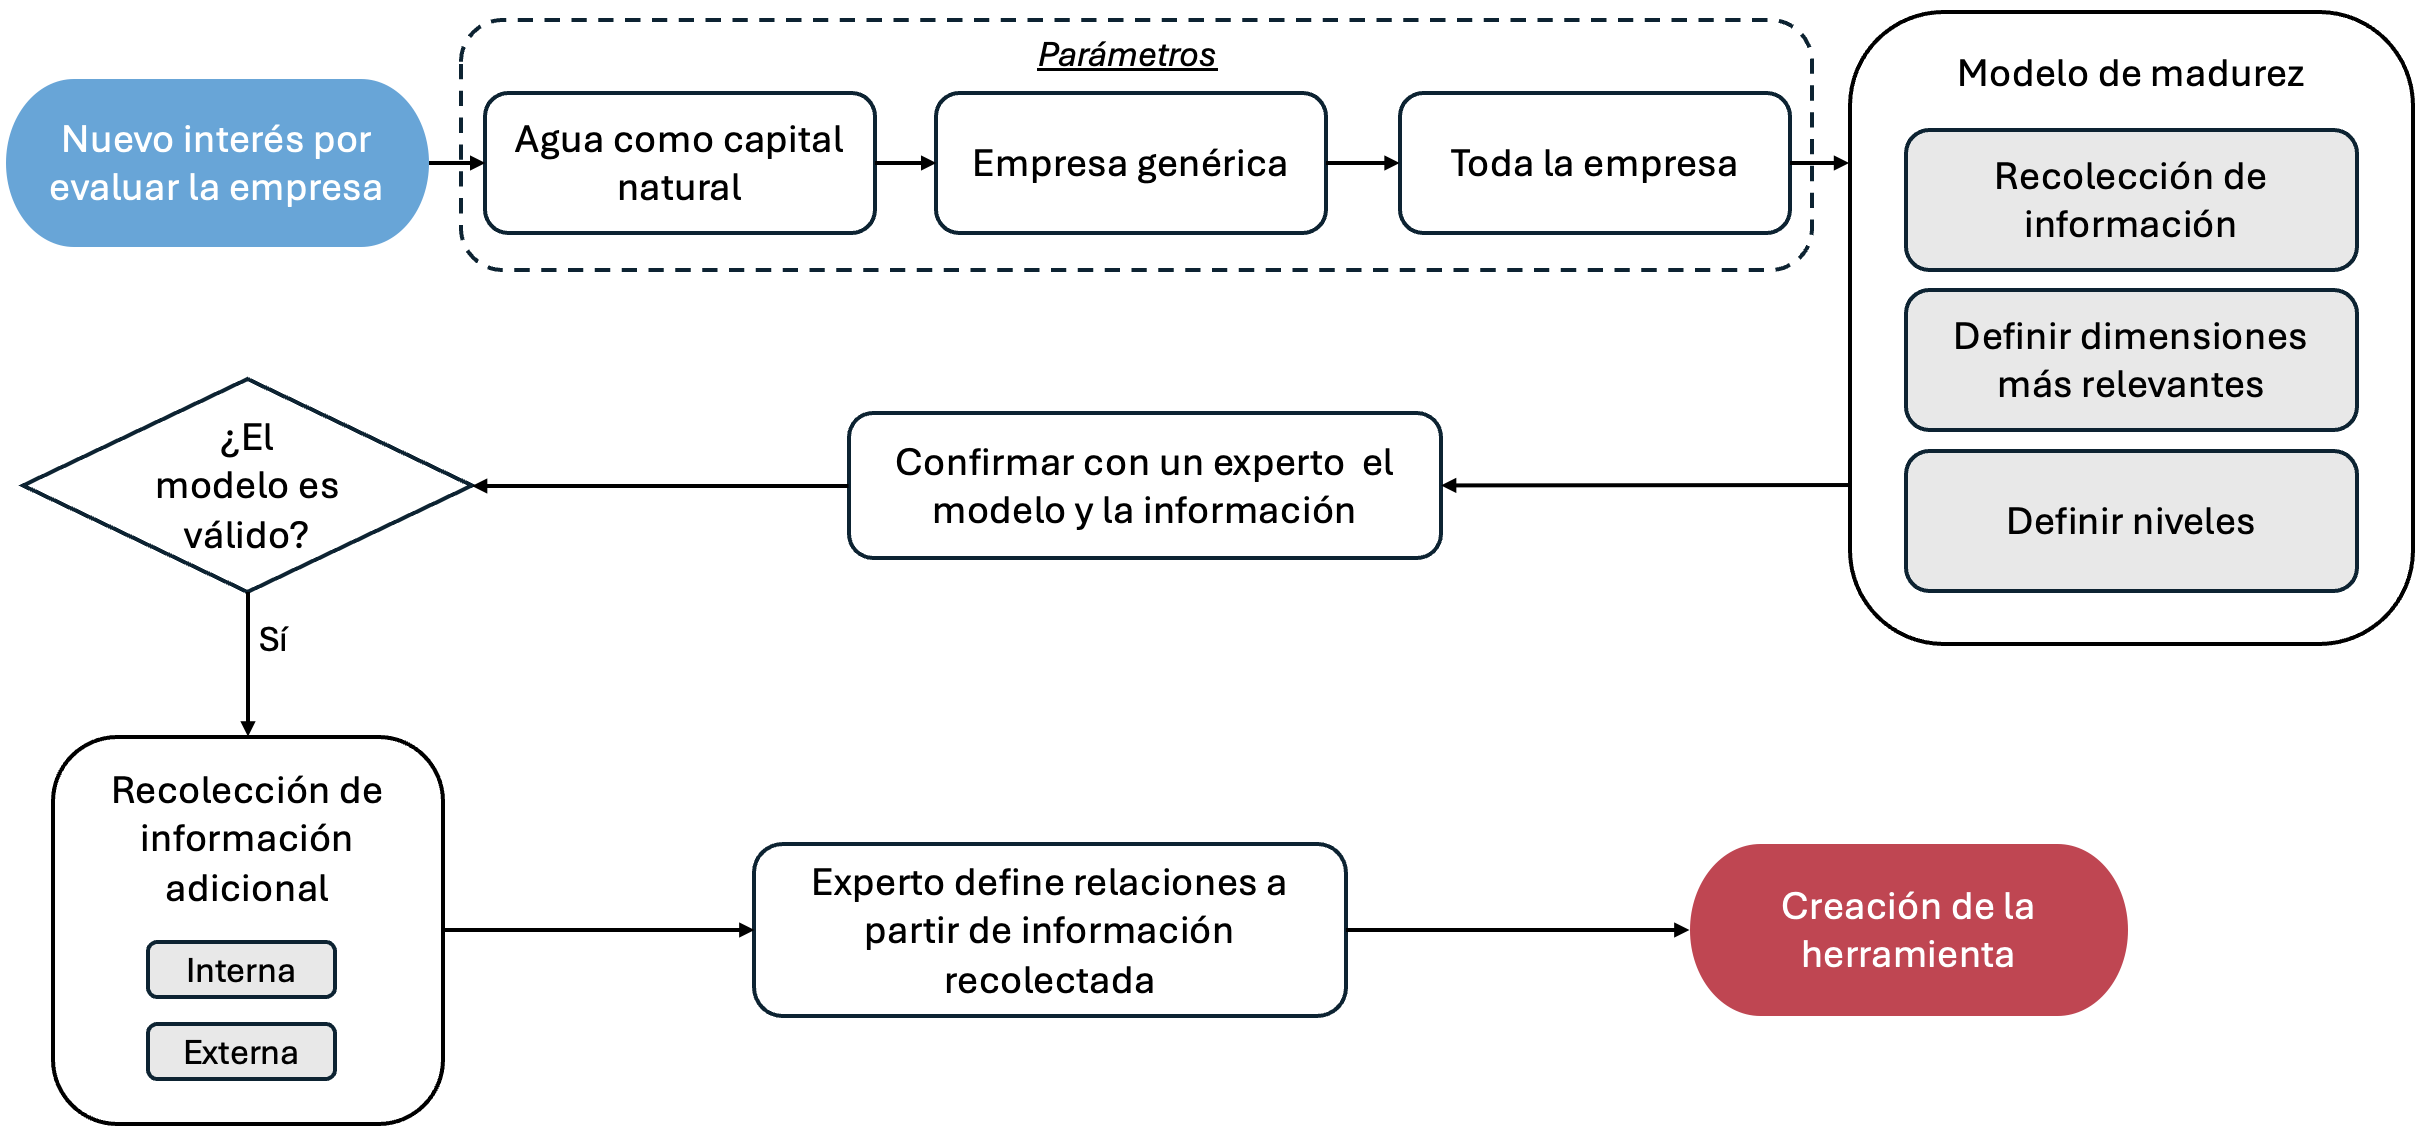
\includegraphics[scale=0.25]{images/5-implementacion/estrategia-negocio-agua.png}
    \caption{Flujo de la estrategia Negocio-Agua}
    \label{fig:estrategia-negocio-agua}
\end{figure}

Luego de haber definido los parámetros que serán evaluados en esta estrategia, se procede a crear el modelo de madurez que evalué a la empresa. El modelo de madurez fue realizado utilizando la metodología descrita en la sección \ref{sec:desarrollo-diseno}. \nameref{sec:desarrollo-diseno} , utilizando las fuentes de información descritas en la sección \ref{subsec:recoleccion-informacion}. \nameref{subsec:recoleccion-informacion}. Este modelo está compuesto por siete dimensiones que evalúan a la empresa y cuatro niveles posibles de clasificación.  En la siguiente sección se describirá en mayor detalle el modelo de madurez y sus componentes.

La información adicional que se requirió para completar el modelo y la estrategia fue principalmente información externa. Como dicho en la sección \ref{sec:desarrollo-diseno}. \nameref{sec:desarrollo-diseno}  la información externa hace referencia a la información acerca del concepto a evaluar, en este caso el agua como capital natural, que el experto necesita para poder determinar las relaciones. En especial, la información adicional recolectada estuvo relacionada a indicadores de agua, servicios, funciones y gestiones ecosistémicas relacionadas al agua. Adicionalmente, para mayor robustez del modelo, la experta M.A. Parra sugirió implementar la metodología \textit{Analytic Hierarchy Process} la cual será explicada en la siguiente sección. Finalmente, luego de tener toda la información, la validación del modelo, las relaciones entre el negocio y el agua establecidas se puedo hacer la creación de la herramienta. La implementación de la herramienta fue hecha a través de una aplicación web. El objetivo de la herramienta es desarrollar e implementar el modelo generado por la estrategia para determinar el nivel de madurez de la empresa, al mismo tiempo que se visualiza su relación con el agua a partir de la información proporcionada por la misma empresa. Más detalles e imágenes de la aplicación web serán mostrados en la sección \ref{subsec:implementacion-desarrollo-herramienta}. \nameref{subsec:implementacion-desarrollo-herramienta}.

\subsection{Descripción de la implementación} \label{subsec:descripcion-implementacion}

En esta sección se explicará cada componente de la estrategia en detalle. Primero, se explicará el modelo de madurez generado por la estrategia y todos sus componentes. Luego, se procederá a explicar la metodología \textit{Analytic Hierarchy Process}, la cual fue implementada para darle mayor robustez al modelo. Por último, se mostrarán las relaciones entre el negocio y el agua que se generaron y la manera en que fueron establecidas.

\subsubsection{Modelo de madurez}
Un modelo de madurez según \textcite{poppelbu-2011} en su artículo \textit{What Makes a Useful Maturity Model? A Framework of General Design Principles for Maturity Models and Its Demonstration in Business Process Management} es:

\hfill
\par
\leftskip=0.35in \rightskip=0.35in
[…] un marco estructurado que describe las etapas de evolución y mejora en un área de interés particular, como procesos, capacidades o entidades. Típicamente consiste en una serie de niveles o etapas que representan niveles crecientes de madurez o sofisticación. Los modelos de madurez se utilizan para evaluar el estado actual de una organización o sistema, identificar áreas de mejora y proporcionar una hoja de ruta para avanzar hacia niveles más altos de madurez.

\hfill
\par
\leftskip=0in \rightskip=0in

En el caso de este documento, el modelo de madurez (Figura \ref{fig:modelo-madurez}) originado de la estrategia Negocio-Agua, determina el nivel de madurez de una empresa en cuanto a sus conocimientos y acciones sobre las dependencias e impactos que tiene sobre el agua como capital natural. Los cuatro niveles que componen este modelo de madurez están basados en los niveles del proyecto \textit{Valuing Water Finance Initiative Benchmark} \parencite{ceres-2023B}.

\begin{figure}[H]
    \centering
    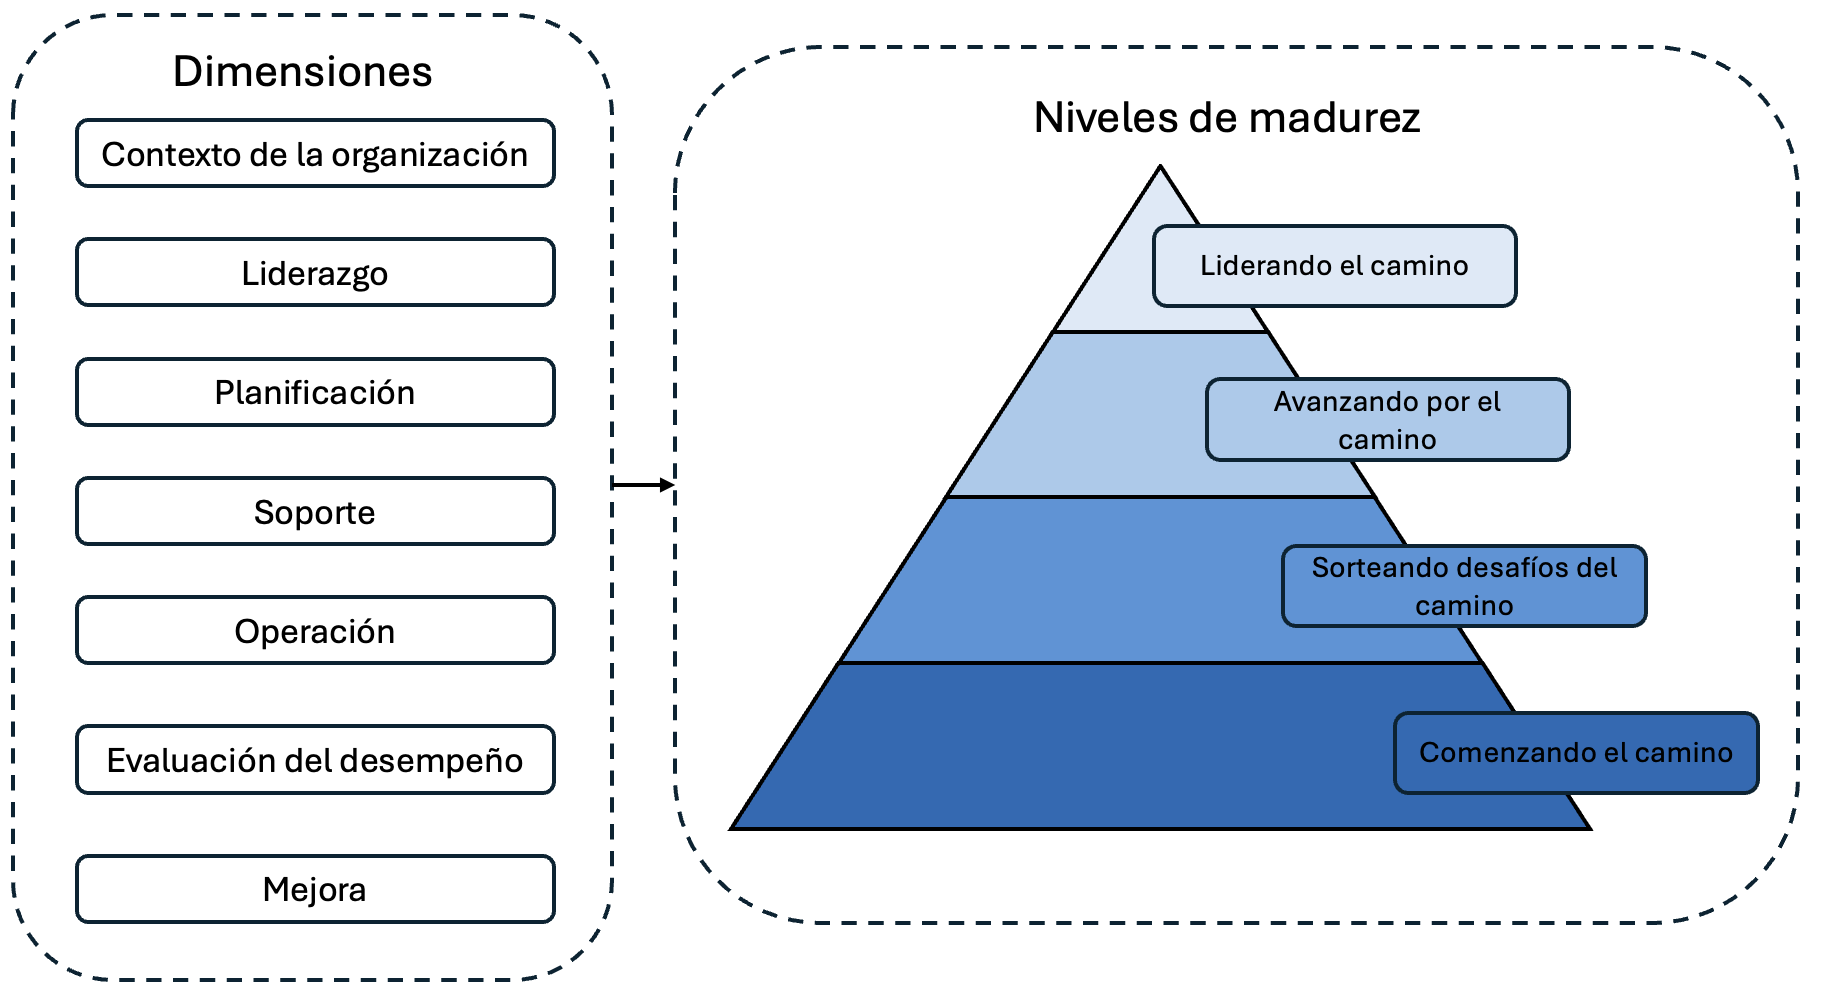
\includegraphics[scale=0.4]{images/5-implementacion/modelo-madurez.png}
    \caption{Modelo de madurez}
    \label{fig:modelo-madurez}
\end{figure}

El primer nivel del modelo de madurez de la estrategia Negocio-Agua se llama Comenzando el camino. En este nivel la empresa todavía está en etapas preliminares para lograr comprender y actuar sobre las dependencias e impactos que tiene sobre el agua. En el siguiente nivel de madurez denominado ‘Sorteando desafíos del camino’ la empresa ya ha comenzado a comprender y actuar sobre las dependencias e impactos que tiene sobre el agua, sin embargo, grandes esfuerzos se deben seguir haciendo para mejorar. En el tercer nivel de madurez, ‘Avanzando por el camino’, la empresa ya logra comprender y actuar sobre las dependencias e impactos que tiene sobre el agua casi en su totalidad. En algunos casos ya empieza hacer una referencia para otras empresas. Por último, en el nivel de madurez ‘Liderando el camino’ la empresa ya logra comprender y actuar sobre las dependencias e impactos que tiene sobre el agua en su totalidad. En la mayoría de los casos es una referencia para otras empresas, además de tener programas y proyectos adicionales a favor del agua. En la tabla a continuación se muestra el puntaje mínimo y máximo por nivel. El sistema de puntuación será explicado a lo largo de esta sección.


\begin{table}[H]
    \centering
    \begin{tabular}{p{7cm} | p{2cm} | p{2cm}}
        \textbf{Nivel} & \textbf{Mínimo} & \textbf{Máximo}\\
        \hline\hline
        Comenzando el camino & 0 & 30 \\
        \hline
        Sorteando desafíos del camino & 31 & 50\\
        \hline
        Avanzando por el camino & 51 & 75\\
        \hline
        Liderando el camino & 76 & 100 \\
        \noalign{\global\arrayrulewidth=1pt} 
        \hline
    \end{tabular}
    \caption{Puntaje mínimo y máximo por nivel de madurez}
    \label{tab:niveleles-min-max}
\end{table}

El sistema de puntos está determinado a partir de las siete dimensiones que se evalúan a la empresa. Las dimensiones fueron definidas a partir de la ISO 14001 Sistemas de Gestión Ambiental – Requisitos con orientación para su uso \parencite{iso-2015}. Como se puede ver en la Figura \ref{fig:modelo-madurez} la primera dimensión es ‘Contexto de la organización’. Esta dimensión busca comprender el contexto en el que opera la organización, incluyendo las necesidades y expectativas relacionadas con el agua como servicio ecosistémico. Es crucial para determinar los objetivos y el alcance de la gestión del agua. Luego está ‘Liderazgo’ la cual evalúa a la alta dirección\footnote{Alta dirección: persona o grupo de personas que dirige y controlan una organización al más alto nivel \parencite{iso-2015}.}. Esta debe mostrar un compromiso claro con la gestión del agua como servicio ecosistémico, estableciendo políticas y asignando responsabilidades para garantizar su efectividad. La siguiente dimensión, ‘Planificación’, evalúa establecer objetivos claros relacionados con la gestión del agua, considerando los riesgos, oportunidades y dependencias asociadas. También implica evalúa la integración de acciones específicas para alcanzar los objetivos ambientales relacionados con el agua en los procesos de negocio de la organización. La cuarta dimensión, ‘Soporte’, evalúa si la organización proporciona los recursos necesarios y se asegura de que su personal tenga las competencias adecuadas para llevar a cabo la gestión del agua como servicio ecosistémico. Además, evalúa si los canales de comunicación son efectivos interna y externamente.  Internamente hace referencia a comunicaciones que deberían ocurrir dentro de la misma empresa, mientras que, externamente hace referencia a comunicaciones con, por ejemplo, proveedores o clientes. La siguiente dimensión, ‘Operación’, hace referencia a la planificación, implementación y control de los procesos necesarios para cumplir con los requisitos de gestión del agua como capital natural, así como para responder a situaciones de emergencia relacionadas con el agua. La sexta dimensión, ‘Evaluación del desempeño’, incluye la evaluación del seguimiento, medición, análisis y evaluación del desempeño en la gestión del agua como capital natural, con revisiones periódicas por parte de la alta dirección para garantizar la eficacia continua. Finalmente, la última dimensión, ‘Mejora’, incluye la evaluación de la identificación de áreas de mejora, la implementación de acciones correctivas y preventivas, la participación en la restauración y reparación de daños al agua y los ecosistemas, así como el compromiso con la mejora continua en la sostenibilidad ambiental y la protección de los recursos hídricos.

A partir de las siete dimensiones previamente descritas se califica a la empresa para luego determinar el nivel de madurez. Cada dimensión tiene un número de preguntas que evalúan a la empresa (en la sección \ref{apx:preguntas}. \nameref{apx:preguntas} están todas las preguntas hechas con sus respuestas posibles). En la siguiente tabla se podrá ver el número de preguntas y puntos por dimensión.


\begin{table}[H]
    \centering
    \begin{tabular}{p{5cm} | p{4.5cm} | p{4.5cm}}
        \textbf{Dimensión} & \textbf{Núm. Preguntas} & \textbf{Puntos disponibles}\\
        \hline\hline
        Contexto de la organización & 12 & 20 \\
        \hline
        Liderazgo & 7 & 10 \\
        \hline
        Planificación & 13 & 31\\
        \hline
        Soporte & 12 & 22\\
        \hline
        Operación & 5 & 7\\
        \hline
        Evaluación del desempeño & 13 & 28 \\
        \hline
        Mejora & 7 & 5\\
        \hline
        \textbf{Total} &  69 & 123\\
        \hline
    \end{tabular}
    \caption{Número de preguntas y puntos disponibles por dimensión}
    \label{tab:num-preguntas-puntos-dimension}
\end{table}

Estas preguntas son de diferentes estilos, existen preguntas de si-no, escogencia única y múltiple. Cada pregunta, además, tiene la opción de No Sabe/ No responde (NS/NR) ya que esta estrategia está dirigida a una empresa genérica. El puntaje de la dimensión es determinado por la respuesta que se da en cada pregunta. Existen diferentes tipos de puntajes de preguntas. Sin embargo, para determinar el puntaje que tenía cada respuesta se pensó en la empresa ideal. Esto quiere decir, se pensaba como la empresa ideal y a partir de ahí se asignaba el puntaje. Por ejemplo, en la pregunta número 21.1, la empresa ideal debería seleccionar a todos los \textit{stakeholders} ya que en la implementación de la estrategia todo el mundo debería ser tomado en cuenta. En siguiente tabla se podrá ver los tipos de preguntas y sus sistemas de calificación. 


\begin{table}[H]
    \centering
    \begin{tabular}{p{5cm} | p{8cm}}
        \textbf{Nombre} & \textbf{Descripción}\\
        \hline\hline
        Binario & Solo una de las opciones disponibles da puntos \\
        \hline
        Si Sabe/Si Responde & Si la respuesta no es NS/NR dará un punto\\
        \hline
        Suma & El número de opciones seleccionadas, que no sean NS/NR, dará puntos.\\
        \hline
        Mejor & Entre todas las opciones existen opciones con más y menos puntos\\
        \hline
        No Puntos & Ninguna opción de la pregunta dará puntos\\
        \hline
    \end{tabular}
    \caption{Tipo de pregunta y su sistema de calificación}
    \label{tab:pregunta-calificacion}
\end{table}

\subsubsection{Metodología: \textit{Analytic Hierarchy Process}}
Luego de tener el puntaje por dimensión para determinar el nivel de madurez, se aplica una ponderación. Esta ponderación se basa en la importancia relativa de cada dimensión en la determinación del nivel de madurez. Es decir, a cada dimensión se le asigna un porcentaje (peso) para determinar el puntaje final. Este peso se determinó utilizando la metodología \textit{Analytic Hierarchy Process} \parencite{bahurmoz-2006}.

La metodología del Proceso Analítico Jerárquico (AHP) es un enfoque estructurado para la toma de decisiones que ayuda a descomponer problemas complejos en componentes más manejables, establecer prioridades y tomar decisiones racionales. Se basa en la comparación de criterios y alternativas a través de matrices de comparación, lo que permite asignar pesos a los criterios y tomar decisiones fundamentadas. 

Para obtener los pesos por dimensión se realizó un taller con cuatro expertos en donde se determinada la importancia relativa. El objetivo de este taller es establecer la importancia de las dimensiones que determinan el nivel de la empresa con respecto a sus dependencias e impactos sobre el agua. La importancia será determinada haciendo una comparación entre cada dimensión. Es decir, la importancia de la 'Dimensión A' relativa a la 'Dimensión B'. A continuación, se puede ver una matriz ejemplo del taller.

\begin{figure}[H]
    \centering
    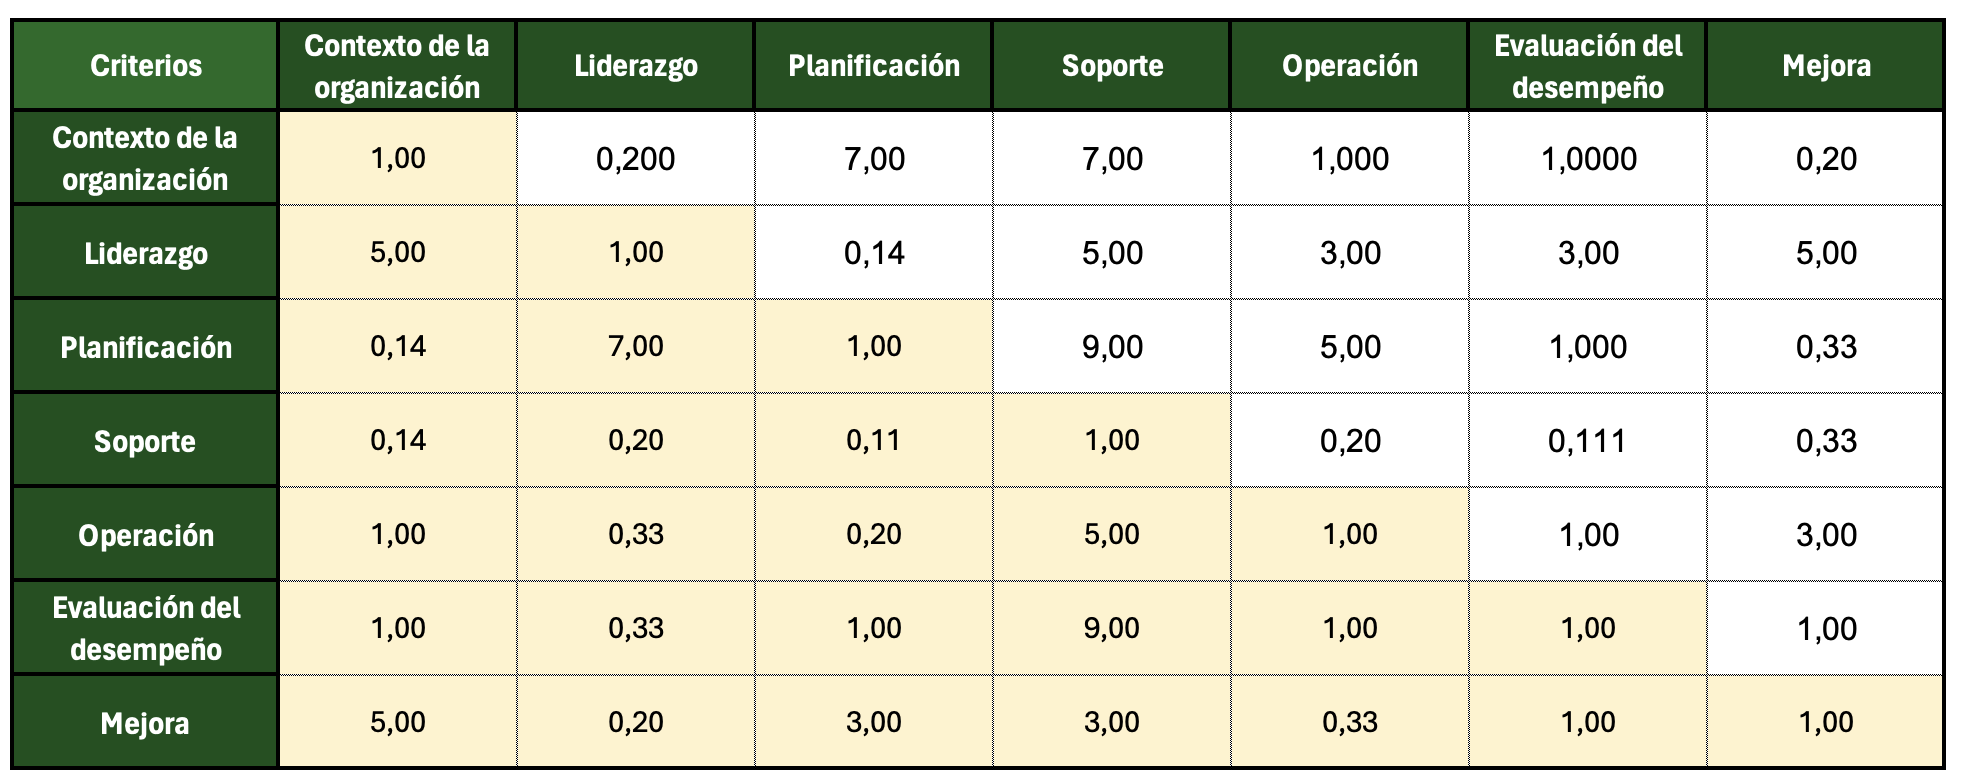
\includegraphics[scale=0.45]{images/5-implementacion/ejemplo-matriz.png}
    \caption{Ejemplo de matriz realizada por experta M.A. Parra}
    \label{fig:ejemplo-matriz}
\end{figure}

Las comparaciones se hacen Fila 1 vs Todas las columnas, luego Fila 2 vs Todas las columnas, etc.  Para determinar la importancia la matriz se lee tal que se haga la pregunta: "¿Qué tan importante es la dimensión i (fila) con respecto a la dimensión j (columna)?". La importancia entre dos dimensiones se determina de la siguiente manera: si es igual de importante = 1; si es levemente más importante = 3; si es mucho más importante = 5; si es demasiado más importante = 7; si es extremadamente más importante = 9. Si el experto cree que la importancia de la dimensión de la fila 1 es menor por un grado N relativa a alguna columna, entonces coloque en la celda correspondiente 1/N. Para obtener los pesos definitivos por dimensión se hizo el promedio de los pesos por dimensión. A continuación, podrá ver los resultados del taller y los pesos por dimensión.


\begin{table}[H]
    \centering
    \begin{tabular}{p{5cm}|p{1.25cm}|p{1.25cm}|p{1.25cm}|p{3.25cm}}
        \textbf{Dimensión} & \textbf{Exp 1} & \textbf{Exp 2} & \textbf{Exp 3} & \textbf{Peso Definitivo} \\
        \hline\hline
        Contexto de la organización & 17\% & 11\% & 34\% & 21\%\\
        \hline
        Liderazgo & 21\% & 25\% & 13\% & 20\%\\
        \hline
        Planificación & 27\% & 13\% & 14\% & 18\%\\
        \hline
        Soporte & 2\% & 18\% & 7\% & 9\%\\
        \hline
        Operación & 8\% & 6\% & 20\% & 11\%\\
        \hline
        Evaluación del desempeño & 11\% & 6\% & 6\% & 8\%\\
        \hline
        Mejora & 14\% & 20\% & 6\% & 14\%\\
        \hline
    \end{tabular}
    \caption{Pesos relativos de las dimensiones por experto}
    \label{tab:pesos-expertos}
\end{table}

\subsubsection{Sistema de puntos}
Luego de obtener los puntos y los pesos relativos por dimensión se puede proceder a obtener el puntaje final que determina el nivel de madurez. En la Ecuación \ref{eq:nivel-madurez} se puede ver cómo se obtiene el puntaje.

\begin{equation} \label{eq:nivel-madurez}
P = (\sum_{i=1}^{7} d_i/t_i \times p_i) \times 100
\end{equation} 

El puntaje final, $P$, es igual a la suma del porcentaje de  puntos obtenidos de cada dimensión $i$, $d_i/t_i$, ponderado por el peso de misma la dimensión, $p_i$. La variable $d_i$ corresponde a los puntos obtenidos en la dimensión $i$, mientras que la variable $t_i$ es la cantidad de puntos posibles de la dimensión $i$.

\subsubsection{Relación entre el negocio y el agua}
Además de determinar el nivel de madurez de una empresa, la estrategia también busca concientizar a las empresas sobre sus actuales relaciones con el agua. Estas relaciones se basan en los indicadores que la empresa actualmente mide o contempla en los reportes que realiza acerca del agua como capital natural dentro de su negocio. En específico, con qué SSEE, funciones y gestiones ecosistémicas se relacionan los indicadores de la empresa. Estas relaciones fueron determinadas por los expertos M.A. Parra y M. Murcia, los cuales utilizaron las siguientes referencias: \textit{Guidelines for identifying business risks and opportunities arising from ecosystem change: Version 2.0} (Hanson et al., 2012) y \textit{A typology for the classification, description and valuation of ecosystem functions, goods and services} (De Groot et al., 2002). Los expertos fundamentaron sus respuestas en estas dos referencias debido al elevado nivel de aceptación que tienen en la industria y a su amplia citación en diversos artículos. El objetivo principal de establecer estas relaciones es poder concientizar a las empresas de que los procesos que ellos realizan tienen dependencias y generan impactos sobre los SSEE, funciones y procesos ecológicos asociados al agua.  En la sección de Anexos, podrá encontrar los indicadores y sus respectivas relaciones. 

Establecer las relaciones entre el negocio y el agua, en especial entre los indicadores que utiliza la empresa y las gestiones ecosistémicas cobra importancia en Colombia para seguir la \acrfull{pngibse}. Según el \textcite{ministerio-de-ambiente-y-desarrollo-sostenible-2012},

\hfill
\par
\leftskip=0.35in \rightskip=0.35in
\acrshort{pngibse} será la que enmarque y oriente conceptual y estratégicamente todos los demás instrumentos ambientales de gestión (políticas, normas, planes, programas y proyectos), existentes o que se desarrollen, para la conservación de la biodiversidad en sus diferentes niveles de organización, además de ser base de articulación intersectorial y parte fundamental en el desarrollo del país.

\hfill
\par
\leftskip=0in \rightskip=0in
Es por esto por lo que es muy importante que las empresas entiendan y conozcan las relaciones que existen entre su negocio y los diferentes componentes del ecosistema. Esto incluye, además, todos los capitales naturales, SSEE, funciones ecosistémicas, etc. Entendiendo estas relaciones, va a ser la forma principal en la que las empresas podrán seguir mejorando sus estados actuales. Además, podrá minimizar los costos adicionales generados por reparaciones y daños, si desde un principio entienden las relaciones tal que puedan seguir las políticas, normas, planes, programas y proyectos. 

\subsubsection{Indicadores}
Además de establecer las relaciones con el agua, los indicadores también son una fuente de información para evaluar una empresa (\ref{apx:indicadores}. \nameref{apx:indicadores}). En especial, evaluar los datos y las fuentes de información y la calidad de los atributos que mide las empresas. Para esto, la estrategia evalúa la granularidad, frecuencia, comparabilidad, fuente, tipo, \textit{Sciene Based Target} (SBT)\footnote{\textit{Science Based Target}: Los objetivos basados en la ciencia proporcionan una vía claramente definida para que las empresas reduzcan las emisiones de gases de efecto invernadero (GEI), ayudando a prevenir los peores impactos del cambio climático y el crecimiento empresarial a prueba de futuro \parencite{science-based-targets-no-date}.} y validación externa. En la siguiente tabla se podrá ver las preguntas que se hacía por atributo de calidad del indicador y sus opciones.


\begin{table}[H]
    \centering
    \begin{tabular}{p{3cm} | p{7cm} | p{4.5cm}}
        \textbf{Dimensiones} & \textbf{Pregunta} & \textbf{Opciones} \\
        \hline\hline
        Granularidad & Seleccione el nivel de granularidad de los datos&País-Departamento-Municipio-Cuenca-NS/NR\\
        \hline
        Frecuencia & Seleccione la frecuencia de los datos utilizados para armar/calcular los indicadores&Diaria-Semanal-Mensual-Bimestral-Semestral-Anual-NS/NR\\
        \hline
        Comparabilidad & ¿Sus datos han sido comparados con otros datos externos?&SI-NO-NS/NR\\
        \hline
        Fuente & ¿Cuál es la fuente principal de los datos utilizados para armar/calcular los indicadores?& Datos primarios-Datos secundatios-NS/NR\\
        \hline
        Tipo & ¿Qué tipo de indicador es?&Cualitativo-Cuantitativo-NS/NR\\
        \hline
        SBT & ¿Sus datos son \textit{Science Based Targets} (SBT)?& SI-NO-NS/NR\\
        \hline
    \end{tabular}
    \caption{Atributos evaluados de los indicadores}
    \label{tab:atributos-indicadores}
\end{table}

\subsubsection{Servicios Ecosistémicos}
La estrategia también le permite a la empresa que tiene un mayor grado de conocimiento evaluar las dependencias e impactos sobre los servicios ecosistémicos asociados a los indicadores medidos. Esto permite una mayor profundización en la estrategia y, además, a aquellas empresas que no sabían acerca del nivel de dependencia (bajo, medio o alto) y el tipo de impacto (positivo o negativo) que tenían sobre los servicios ecosistémicos asociados a los indicadores medido o contemplados, les hace reflexionar y enterarse de información que deberían tener en cuenta. 


\subsection{Implementación y desarrollo de la herramienta} \label{subsec:implementacion-desarrollo-herramienta}

En esta sección se explicará el desarrollo e implementación del modelo generado por la estrategia en una herramienta que permita determinar el nivel de madurez de la empresa, al mismo tiempo que se visualiza su relación con el agua a partir de la información proporcionada por la misma empresa. La herramienta se desarrolló en una aplicación web que utiliza MongoDB para almacenar los datos, Render para desplegar la aplicación y Dash Plotly como librería principal de Python para crear la aplicación y sus servicios. En el siguiente diagrama se podrá ver la relación entre los componentes previamente mencionados. 

\begin{figure}[H]
    \centering
    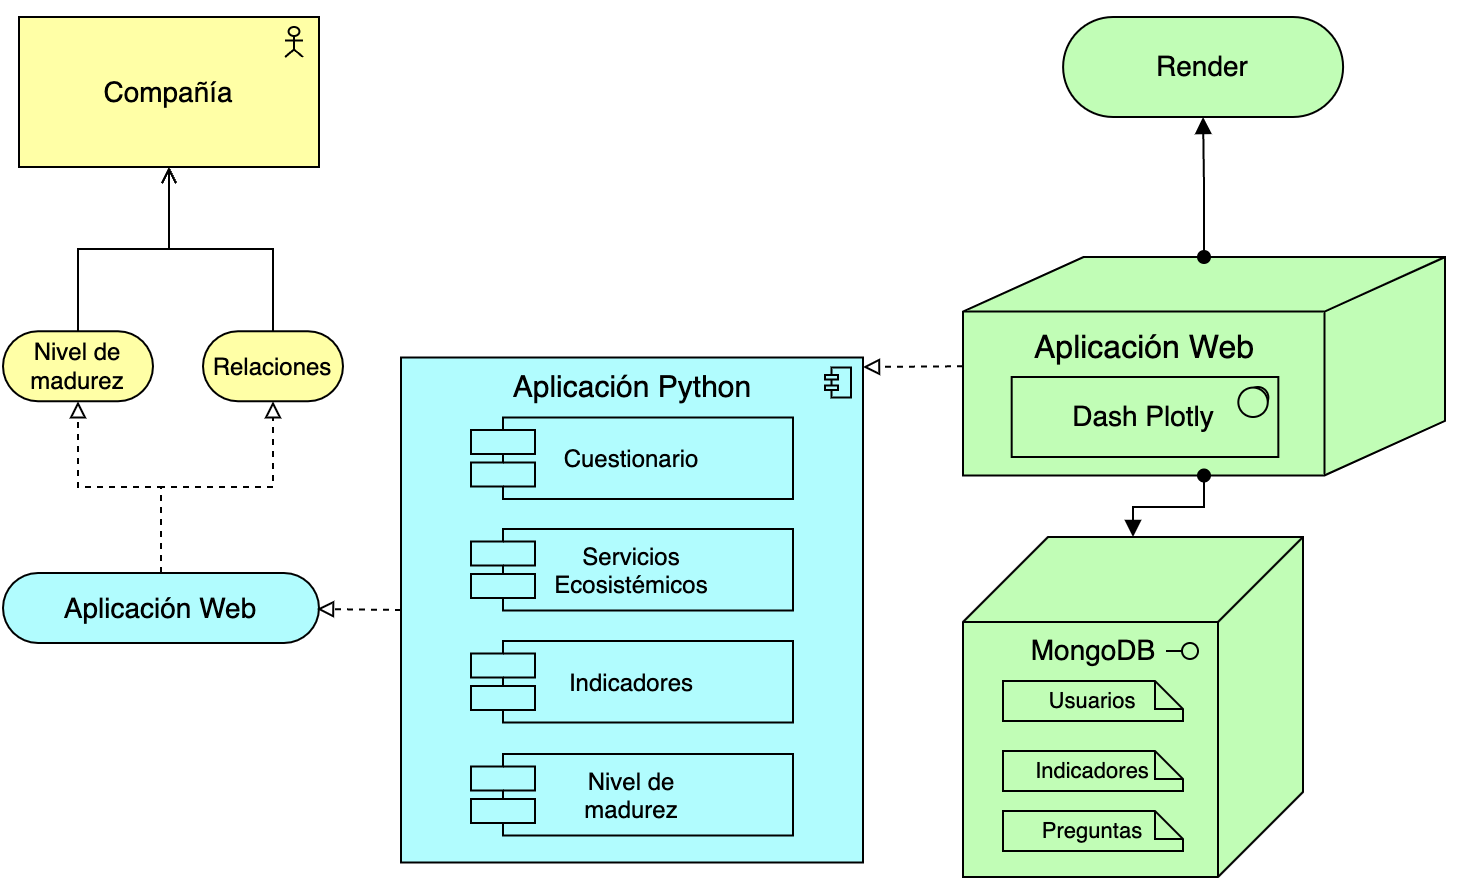
\includegraphics[scale=0.45]{images/5-implementacion/diagrama-archimate.png}
    \caption{Diagrama archimate de la aplicación web}
    \label{fig:archimate-app-web}
\end{figure}

A través de una serie de preguntas, se buscará determinar el nivel de madurez de la empresa con respecto a las dependencias e impactos que tiene sobre el agua. La aplicación web tiene los siguientes objetivos:

\begin{enumerate}
    \item Determinar el nivel de madurez a partir de la evaluación del conocimiento y acciones que tiene la empresa acerca de las dependencias y los impactos sobre el agua.
    \item Entender, de las dimensiones a evaluar, cuál es la mejor dimensión actualmente que tiene la empresa.
    \item Exponer a la empresa, según los indicadores que miden, cuáles servicios y funciones ecosistémicos deben contemplar en los reportes relacionados con el agua.
\end{enumerate}

En la Figura \ref{fig:paso-paso-app} se puede ver el paso a paso de cómo se pueden cumplir con los tres objetivos anteriormente mencionados. En el primer paso, ‘Cuestionario’, la empresa deberá responder un conjunto de preguntas relacionadas a los conocimientos y acciones que actualmente está haciendo en relación con las dependencias e impactos sobre el agua. En el siguiente paso, ‘Indicadores’, la empresa deberá seleccionar los indicadores que actualmente estén midiendo o contemplando en reportes relacionados al agua. Luego, en el paso ‘Nuevos indicadores’, la empresa podrá ingresar sus propios indicadores, que no encontró en la anterior sección, a la herramienta. A partir del segundo paso, en el paso ‘Servicios Ecosistémicos, la empresa podrá determinar el nivel de dependencia (bajo, medio, alto) y el tipo de impacto (positivo, negativo) que tiene sobre los servicios ecosistémicos. En el quinto paso, ‘Funciones Ecosistémicas’, la empresa podrá ver una visualización de la relación entre indicadores, servicios y funciones ecosistémicos, para entender la importancia en la relación entre el negocio y el agua y sus servicios ecosistémicos. Finalmente, en el último paso, ‘Resultados’, la empresa podrá saber cuál es su nivel de madurez, su puntaje obtenido, su mejor dimensión, el puntaje y descripción por dimensión y unas gráficas descriptivas para los indicadores escogidos. En la sección \ref{apx:imagenes-app-web}. \nameref{apx:imagenes-app-web}, están las imágenes para cada uno de los pasos anteriormente mencionados.

\begin{figure}[H]
    \centering
    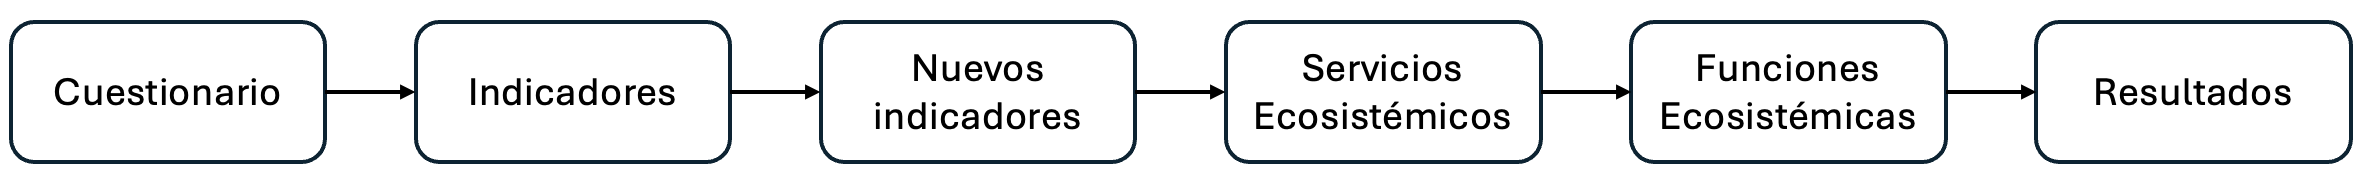
\includegraphics[scale=0.4]{images/5-implementacion/paso-a-paso-app.png}
    \caption{Paso a paso de la aplicación}
    \label{fig:paso-paso-app}
\end{figure}

En la Figura \ref{fig:resultados-nivel-madurez} se ve un resultado ejemplo de la aplicación. En la primera fila, luego del encabezado, se ven los tres primeros resultados. El primer (1) resultado muestra el nivel de madurez obtenido, en este caso 'Sorteando desafíos del camino'. El siguiente resultado (2) muestra el puntaje obtenido, el cual define el nivel de madurez mencionado. El tercer (3) resultado en esta fila muestra la mejor dimensión obtenida por la empresa ('Contexto de la organización').

\begin{figure}[H]
        \centering
        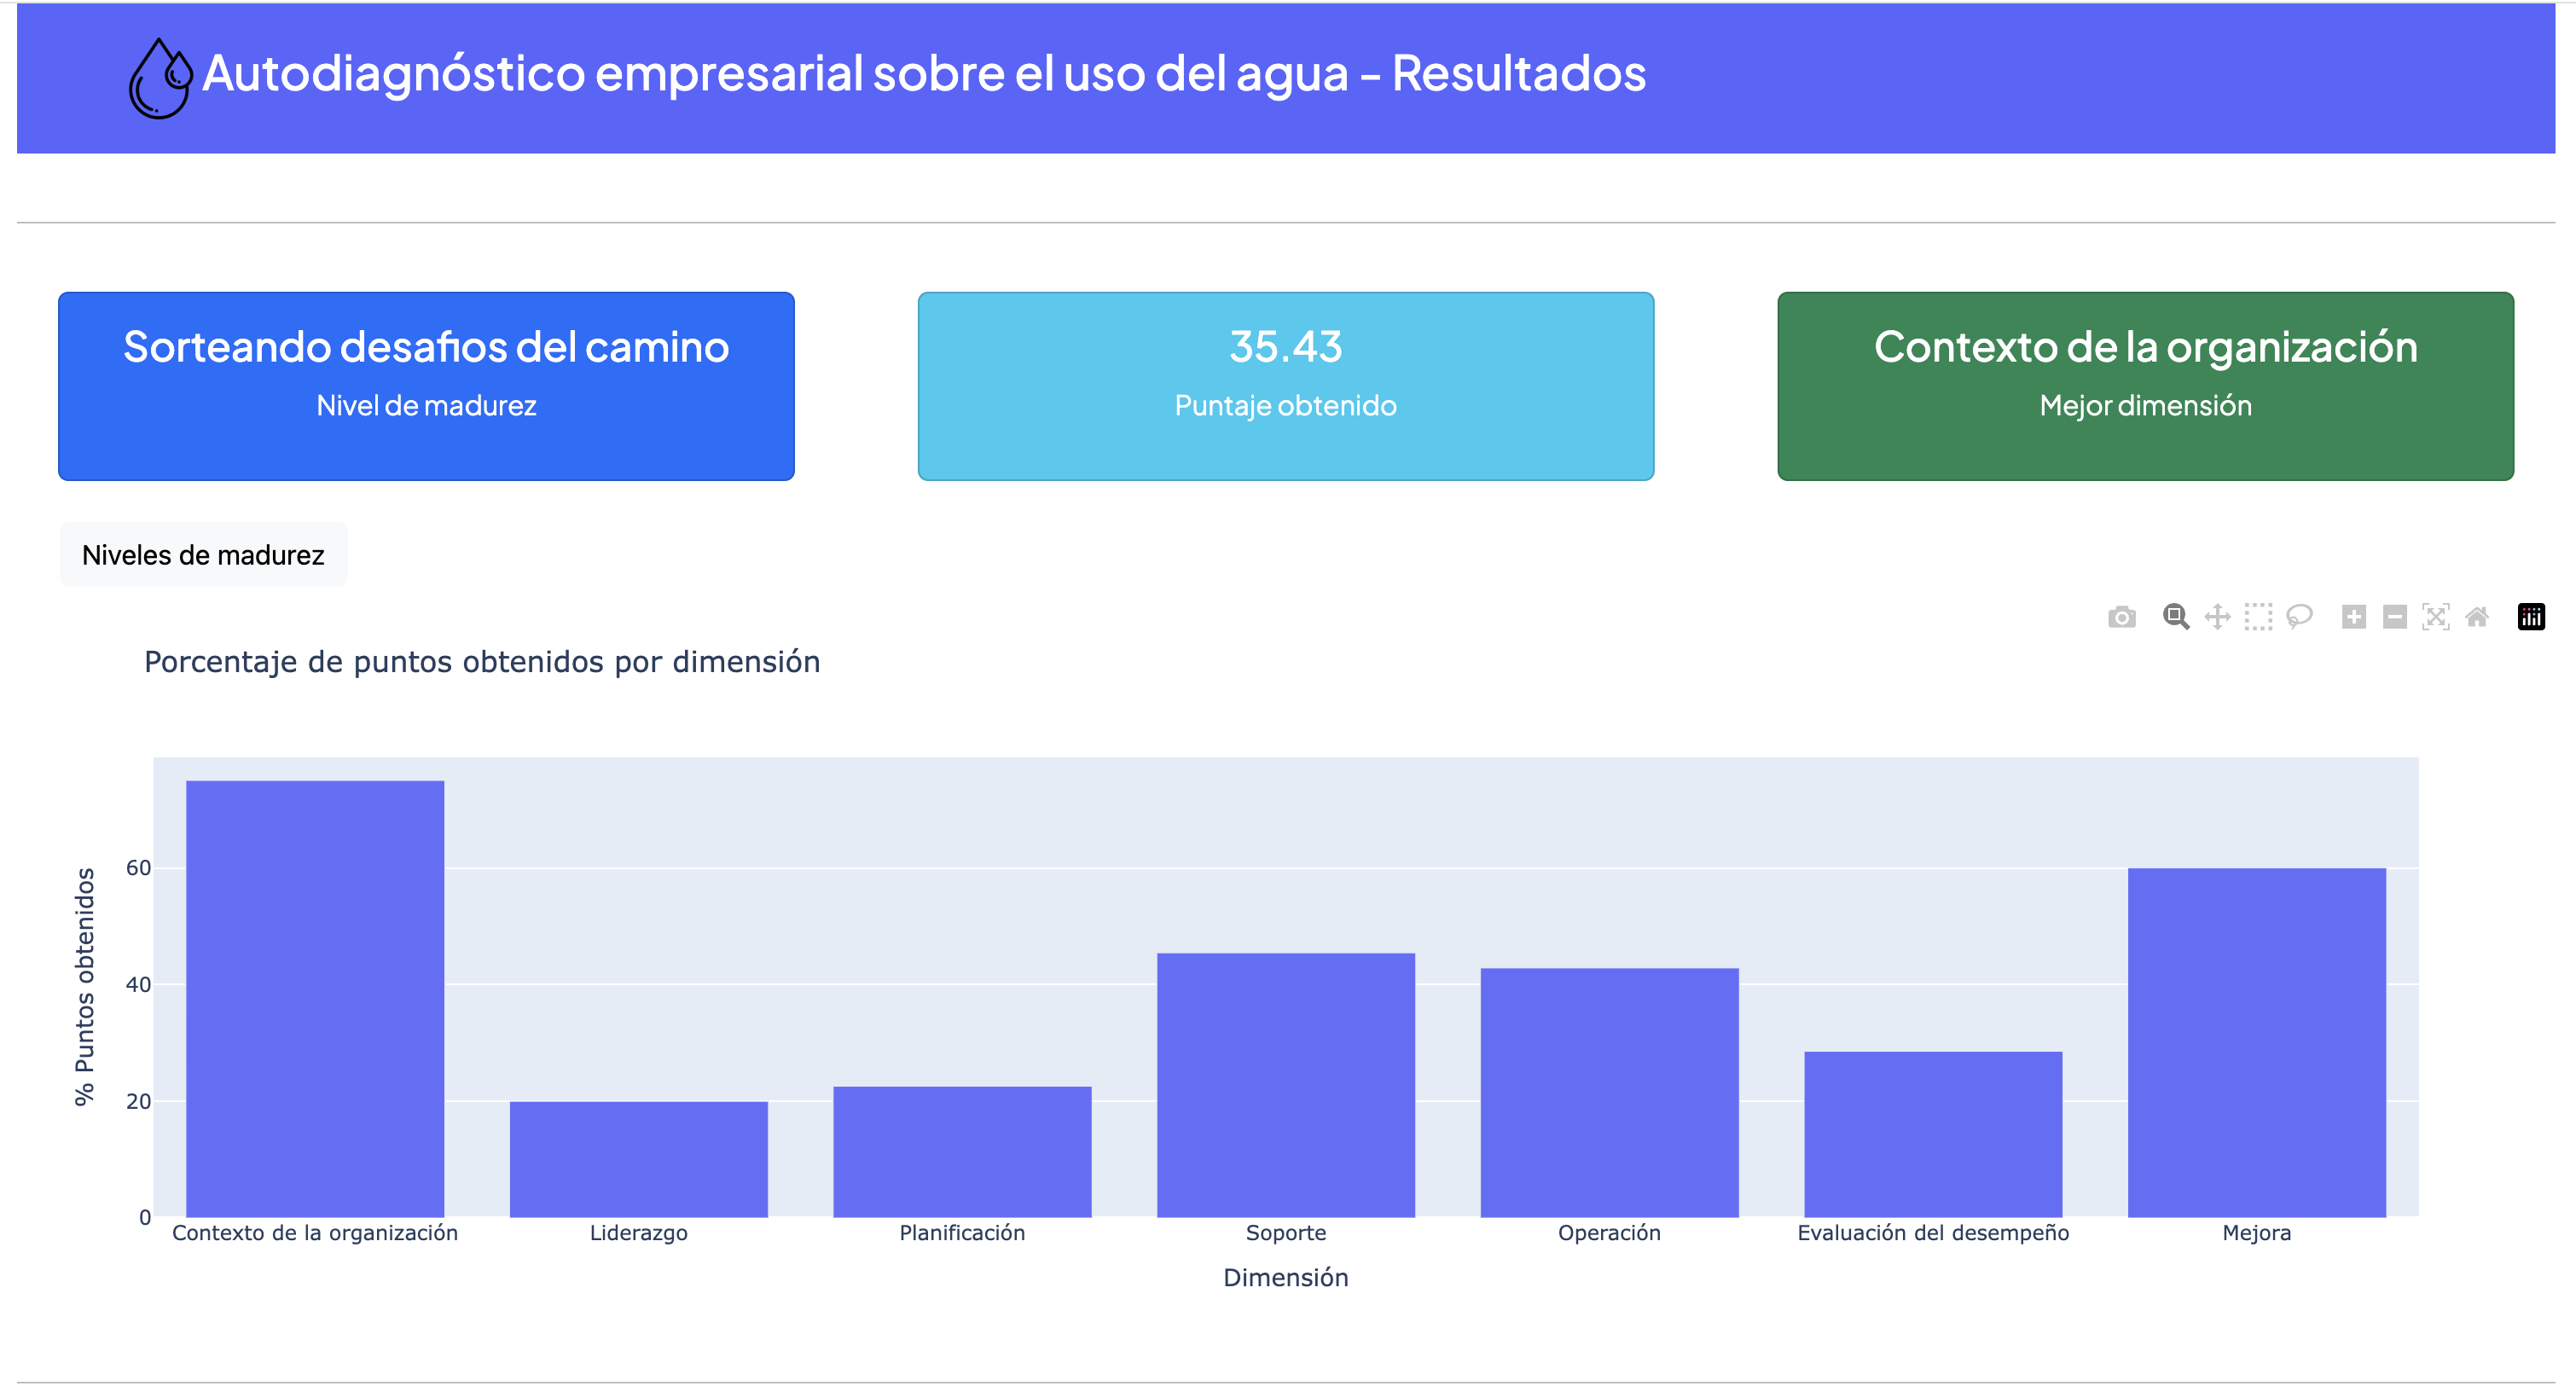
\includegraphics[scale=0.25]{images/99-aplicacion-web/8-mm.png}
        \caption{Resultado-Nivel de madurez de la empresa}
        \label{fig:resultados-nivel-madurez}
\end{figure}

En la gráfica dentro de la Figura \ref{fig:resultados-nivel-madurez}, se observa el porcentaje de puntos obtenidos (eje vertical) para cada dimensión (eje horizontal). Para el 'Contexto de la organización', se obtuvo alrededor del 70\% de los puntos. Esto indica que la empresa conoce su estado actual y sus necesidades; sin embargo, podría mejorar en la determinación de los objetivos y el alcance de la gestión del agua de manera correcta. En la dimensión 'Liderazgo', se evidencia que la alta dirección no muestra un compromiso claro con la gestión del agua, ya que no establece políticas ni asigna responsabilidades para garantizar su efectividad. De manera similar, en la dimensión 'Planificación', con un bajo porcentaje de puntos obtenidos (aproximadamente 23\%), los objetivos no se establecen claramente en relación con la gestión del agua, considerando los riesgos, oportunidades y dependencias asociadas. Para la dimensión 'Soporte', con alrededor del 45\% de los puntos posibles, la empresa debe asegurar que su personal tenga mayores competencias y mejores recursos para llevar a cabo la gestión del agua como servicio ecosistémico. Además, debe establecer canales de comunicación efectivos, tanto internos como externos, relacionados con la gestión del agua. En la dimensión 'Operación', al obtener casi el 42\% de los puntos posibles, la empresa necesita mejorar significativamente en la planificación, implementación y control de los procesos necesarios para cumplir con los requisitos de gestión del agua como servicio ecosistémico, así como en la respuesta a situaciones de emergencia relacionadas con el agua. Según la gráfica, la empresa tiene mucho por mejorar en el seguimiento, medición, análisis y evaluación del desempeño en la gestión del agua, con revisiones periódicas por parte de la alta dirección para garantizar la eficacia continua, ya que obtuvo solamente el 30\% de los puntos posibles en la dimensión 'Evaluación del desempeño'. Finalmente, la empresa debe mejorar sustancialmente en la identificación de áreas de mejora, implementación de acciones correctivas y preventivas, y debe tener una mayor participación en la restauración y reparación de daños al agua y los ecosistemas ya que obtuvo el 50\% de los puntos posibles. 


